\documentclass[titlepage]{article}
\usepackage[preprint]{nips_2018}
\usepackage[utf8]{inputenc} % allow utf-8 input
\usepackage[T1]{fontenc}    % use 8-bit T1 fonts
\usepackage{hyperref}       % hyperlinks
\usepackage{url}            % simple URL typesetting
\usepackage{booktabs}       % professional-quality tables
\usepackage{amsfonts}       % blackboard math symbols
\usepackage{nicefrac}       % compact symbols for 1/2, etc.
\usepackage{microtype}      % microtypography
\usepackage{graphicx}
\usepackage{subcaption}
\bibliographystyle{plainnat}
\title {
Sentiment Analysis in Twitter Context: \\Incorporating Part-of-Speech Tags as Features \\ into a MaxEnt Classifier}


\author{%
  Final Report \\
  Olena~Vyshnevska \\
  Student ID: 798561 \\
  University of Potsdam \\
  \texttt{vyshnevska@uni-potsdam.de} \\
  \textbf{} \\
  Working Group: \\
  Rafi Abdoule Latif \\
  Patrick Kahardipraja}

\begin{document}

\maketitle

\begin{abstract}
The focus of this project is to analyse if tagging words with Part-of-Speech (POS) categories can improve machine learning-based Sentiment Analysis (SA) of tweets. We iteratively searched for optimal strengths for different combinations of POS categories. The experiments illustrate that including POS categories as features slightly increase the performance of a Bag-of-Words (BOW) Maximum Entropy (MaxEnt) classifier. However the Term Frequency - Inverse Document Frequency (TFIDF) classifier outperforms both BOW, POS, and POS-induced BOW.
\end{abstract}

\newpage
\setcounter{page}{1}

\section{Introduction}

%W hat was the topic of your group\'s project, your approach and main results?
Social platforms such as Twitter provide large amounts of data, which can be leveraged by SA classifiers to quantify and categorise opinions of people towards a given topic. The project was inspired by the idea that words carry latent features, which can be utilised for more effective SA.

We focused on one such latent feature: POS category of a word. The hypothesis states that sentiment-carrying subjective words can be assigned higher feature weights because their contribution to the sentiment of a tweet is more significant than that of content terms. In other words, we have attempted to reinforce the strength of more discriminative POS categories. 

Furthermore, POS categories allow to distinguish between polysemous and homonymous words. Hence, by introducing POS categories it becomes possible to distinguish between different meanings of graphemes such as  \textit{like}, which carry a positive sentiment as a verb, but are rather neutral as a preposition or a conjunction. 

The learning objectives of the project are the following:
\begin{itemize}
\item To test whether incorporating POS categories as features can benefit SA
\item  If yes, what are the optimal weighting schemes? Which categories are strong indicators of sentiment? How significant are the differences?
\item What problems arise when relying on POS categories as features? Which linguistic phenomena are not captured by POS categories?
\item From the NLP point of view, how such phenomena as emoticons and hashtags can be leveraged to benefit the SA?
\item From the linguistic point of view, will we be able to identify inherent differences between the degrees to which different POS categories influence the SA?
\end{itemize}


The results obtained through this project provide evidence that POS categories as features alone perform worse than BOW and TFIDF classifiers. However, when enriching the BOW model with POS features the performance of the resulted BOW+POS classifier exceeds the results of BOW by circa 1\%. Yet, the TFIDF model outperforms the POS-enriched BOW model by another 1\%. Combining TFIDF and POS, conversely, decreases the performance of TFIDF on its own. Furthermore, we found that emoticons and interjections consistently perform as strong predictors of sentiment. 

\begin{table}[h!]
       \centering
   \begin{tabular}{@{}lllllll@{}}
   \toprule
         & BOW & TFIDF  & POS & BOW+POS & TFIDF+POS & BOW+TFIDF+POS \\ 
             \midrule
Accuracy & 0.6374 & 0.6515 & 0.5869 & 0.6457 & 0.6425  & 0.6440        \\ 
F$_{1}$ macro & 0.6383 & 0.6512 & 0.5874 & 0.6467 & 0.6428  & 0.6448        \\ 
    \bottomrule
\end{tabular}
\caption{Results Overview}
\label{results_overview}
\end{table}


\section{Related Work}
      
      The idea of searching for optimal weighting schemes for POS has its roots in the research by \cite{improving-sa}. By weighting terms the intention is to get further separation between sentiment-carrying words and content words, without completely ignoring entire word categories. The researchers were able to show that the POS model performs 5 points better than the BOW baseline model, achieving the average F$_{1}$ score of 79.20\%. It is worth noting that the dataset used for the experiments consists of 574 documents, divided into two groups -- \textit{positive} and \textit{negative}. It is reasonable to assume that the results would have been different on a dataset of a similar size to ours and with the division into three categories. 
      
       \cite{improving-sa} also came to a linguistically interesting conclusion that while adjectives are strong indicators of sentiment, adverbs can be just as strong. Similarly, \cite{hatz} demonstrate that adjectives are the strongest predictors of sentence subjectivity. However, \citep{thumbs} and \cite{benamara} show that it is misleading to believe that adjectives alone can predict sentiment better than a unigram model. \cite{pos-based-model} suggest to treat adjectives and adverbs equivalently, and therefore group them in one category. \cite{benamara} support the idea that combining adjectives and adverbs improves the performance of unigram models.

Consistent with our findings, \cite{hu} illustrate that emoticons strongly influence the sentiment of a text message. \cite{felbo} further verify the fact that emoticons carry strong sentiment and emotional information. Since emoticons came into wide usage relatively recently, the research is yet to unveil their full potential to affect SA.

\section{Design}


This section explains the concepts that were developed to achieve the learning objectives of the project. Figure \ref{pipeline} located in the appendix depicts our basic design. 


      \paragraph{Data} We used Twitter data from the subtask "Message Polarity Classification", which is part of a SA shared task at the International Workshop on Semantic Evaluation (SemEval) \citep{SemEval}. The data consists of tweets labelled as \textit{positive}, \textit{negative} and \textit{neutral}. The unprocessed dataset consists of approximately 60 000 tweets. 


      \paragraph{Choice of Classifier} Multinomial logistic regression classification method is used for BOW, TFIDF and POS classifiers. Logistic regression estimation was done using limited memory Broyden–Fletcher–Goldfarb–Shanno optimisation algorithm \citep{lbfgs}. The algorithm finds local minimum of an objective function, making use of objective function values and the gradient of the objective function.

Chiefly, the choice of the classifier reflects the purpose of the project -- to extend and to build on the knowledge gained from the course. Working with machine learning classifiers such as MaxEnt allows us to apply the knowledge we gained from working with Naïve Bayes classifiers, while taking a step towards common machine learning methods. 
      
      \paragraph{Baseline}
We chose to implement two baseline classifiers:
\begin{enumerate}
\item a BOW MaxEnt classifier with binary encoding of features, also known as \textit{term presence}
\item a TFIDF MaxEnt classifier 
\end{enumerate} 
      
      The decision to implement a TFIDF classifier in addition to the BOW model is based on the consideration that very frequent terms shadow frequencies of rarer yet more significant terms in a unigram model. TFIDF assigns larger weights to words that are significant for the classification of a particular document  \citep{Wang2018_WordClustering}. This simple yet powerful method yields best results in our project.

      \paragraph{POS Tagger} Twitter data is challenging for automated language processing due to the conversational style of text and the use of non-standard lexical items and syntactic patters. The Stanford POS tagger scores higher than 97.0\% on the Penn Treebank dataset \citep{penntree}, although its performance on Twitter data drops sharply to 83.14\% \citep{comparison-taggers}.
Therefore, we have opted for a POS tagger that is specifically designed to tag Twitter data. \citet{comparison-taggers} demonstrate that ARK tagger, developed by \citet{cmutagger2-paper}, is the most effective currently available non-neural POS tagger specifically developed for labelling Twitter data. Evaluated on three benchmark datasets, it scores between 90.40\% and 93.4\%. 

Furthermore, the tagger creates separate categories for emoticons and hashtags, which allows us to add these to our POS combinations. This has been a very helpful feature, since the majority of the results in our top ten scoring POS-induced classifiers include emoticons.
      
      \paragraph{Weighting Schemes} 
      
      The intention behind feature weighting is to further separate sentiment-carrying categories from words that are less important for SA. Also, by starting the training from various stand points the classifier has a greater chance to find global maxima. After the strength of a category is set, the feature weight is normalised over all POS strengths in the document. Figure \ref{weight} illustrates the formula for calculation weighting schemes. Here, \textit{w} stands for \textit{word}, \textit{d} -- for \textit{document}, and \textit{c} -- for \textit{POS category}.
      
      \begin{figure}[h!]
\centering
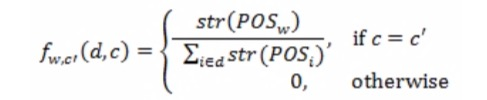
\includegraphics[width=0.4\textwidth]{pics/weight.jpeg}
\caption{Definition of a Weighting Scheme}
\label{weight}
\end{figure}

      
      To find optimal POS strengths, all possible combinations of two sets are constructed: one set consists of POS categories, the other -- of possible weights. For example, the set of POS categories may be \{\textit{adverbs, adjectives, nouns, verbs}\}, and the set of weights may be \{1, 2, 3, 4, 5\}. There are 625 possible combinations in this example. The POS categories that do not belong to the first set receive the weight 0 and are not considered during classification. 
     
     
      \paragraph{OCFS} Orthogonal Centroid Feature Selection (OCFS) was used to reduce the number of features that do not contribute to distinguishing between classes. In its essence, OCFS is aimed at finding features which maximise the distance between the mean feature vectors (centroids) of all classes. In particular, the features that are being reduced are terms.
      
      
      \paragraph{Evaluation Metrics}
Our main evaluation metric is F$_{1}$ score. A classification report is printed after a model finishes predicting. The classification report is a table with precision, recall and F$_{1}$ score metrics for individual classification labels as well as with micro, macro and weighted averages. Additionally, a heat map is created with each prediction to visualise the results.


\section{Implementation}

This section explains the methods the group has used to practically implement the conceptual ideas from the previous section.

      \subsection{Data Processing}
      
     Inspired by Derczynski et al. (2013), we took the following pre-processing steps: we replaced usernames, e-mails, URLs, and numbers with generic tokens; removed HTML tags; fixed escaped unicode characters; and stripped other unwanted characters from words. The steps helped with feature space reduction. We did not lemmatise or stem the words, in order to preserve all the information needed for the POS tagging.
     
     The initial data distribution among the three classes was unequal. Only 18\% of data was labelled \textit{negative}. We have removed documents from both \textit{neutral} and \textit{positive} classes to attain equal amounts of training and testing data in each class. The balancing procedure resulted in a smaller dataset of circa 35000 documents. The data is divided as such: 70\% for training, 10\% for development, 20\% for testing. 

     
     Different spelling correction modules have been examined, such as \textit{pattern} \citep{pattern} and  \textit{ekphrasis} \citep{ekphrasis} with various certainty thresholds. Unfortunately, the spelling correctors introduced more errors than they were helpful. For example, \textit{lol} would be corrected to \textit{Vol}; \textit{black kids gunned down} to \textit{black kiss gunner down}, etc. Furthermore, faulty orthography could potentially have benefits for SA: some groups could intentionally misspell certain terms to convey an affiliation with an ideology. For example, US leftists groups, such the Yippies, substitute \textit{c} with \textit{k}, particularly in the word \textit{Amerika}. Hence, we did not proceed with any further spelling correction. 
     
     \subsection{Modules and Algorithms}

      \paragraph{Classifiers} 
      For baseline as well as for POS model implementations a  \textit{scikit-learn} module has been used \citep{scikit-learn}. The union of models was also implemented with \textit{scikit-learn}.

      \paragraph{OCFS}
      OCFS was implemented according to \citet{ocfs}. Figure \ref{ocfs} in the Appendix presents the algorithm in detail. In our implementation, the feature cutoff number can be specified before each individual training or prediction. In our experiments, the optimal feature cutoff is between 30000 and 40000 features. \cite{improving-sa} found that their optimal feature cutoff was between 1000 and 1500, which can be explained by a very small dataset the researchers used -- only 574 documents.
      
      \subsection{Feature Engineering} 
      On our quest to find the best parameters to reach the highest F$_{1}$ score we have experimented with a variety of model parameters. 

Initially, we have included four categories as suggested by \cite{improving-sa}: adjectives, adverbs, nouns and verbs. Having seen little improvement over the BOW baseline, we have extended the set of POS categories with emoticons, interjections, and hashtags.
     
Moreover, we combined adjectives and adverbs into one category as suggested by \cite{pos-based-model}. We have introduced further grouping methods such as nouns + proper nouns + hashtags; verbs + nominals and verbals + proper nouns and verbals; and emoticons + interjections.

Another influential parameter we experimented with is the union of models. From early on it was clear that POS alone was not a viable model. Hence, we created a pipeline to extract various features in parallel, in our case -- from BOW, TFIDF, and POS models. The features are combined with weights to form one transformer. The weights for each feature in the union can be adjusted before training and predicting.

We have also tried different scales for POS weighting. The training time increases exponentially with every new scalar, therefore the scale was kept at a maximum of 5 to ensure that the running time of one experiment does not exceed four hours.
     
     
     \section{Experiments}
     
     \subsection{Training}
     In order to run an experiment the following arguments have to be specified: the POS categories that will be weighted and if desired, how they are grouped; the upper bound of the weighting scale; the number of features to delete with the OCFS method; weights for the union of models; percentage of the data to use for training; and percentage of the data to use for testing. Such flexibility allows us to easily switch between various configurations for experiments.
     
     Below is an example of a command, which trains 625 models with every possible combination of weights for the specified POS categories on the scale from 1 ot 5. 30000 features will be deleted. Each model will be built with 70\% BOW and 30\% POS. 70\% of data will be used for training, 20\% -- for testing. 

    \begin{verbatim}
      [{"V": ["V"], "A+E": ["A", "E"], "N": ["N"], "R": ["R"]}, 5, 30000,
       {'bow': 0.7, 'pos': 0.3, }, 0.7, 0.2],
    \end{verbatim}

        \subsection{Prediction}
      For prediction the following arguments have to be specified for a desired model: the weights that are assigned to features; number of features to delete; as well as weights for model union. If the model already exists, the classification report for its prediction performance is output. Otherwise, the model is trained, the classification report is printed, and a visualisation of the report is created. Below is an example of a prediction command. 
      
          \begin{verbatim}
      [{'R': 1, 'E': 2, 'A': 4, '!': 4}, 35000, {'bow': 0.5, 'pos': 0.5, }]
          \end{verbatim}
          
          
          
\section{Results}
      
      Table \ref{results_overview} in Section 1 displays the performance of BOW and TFIDF baseline classifiers. Figures \ref{heat_map_bow} and \ref{heat_map_tfidf} in the Appendix illustrate the precision, recall, and F$_{1}$ score for each sentiment class as well as their averages as heat maps.
       
     
Overall, 189 experiments have been carried out by the group. The results are all recorded in the \textit{results} folder in the project directory. Table \ref{top10} provides an overview of the top 10 results we have achieved by incorporating POS information into BOW or BOW+TFIDF classifiers. The suffix \textit{x} represents all suffixes that can fallow a Penn Tree Bank tag, including the lack of a suffix. 
     
\begin{table}[htbp]
  \centering

  \begin{tabular}{*{11}{ll}}
    \toprule
    \multicolumn{6}{c}{POW Strength} & & \multicolumn{3}{c}{Model Union} \\
    \cmidrule(lr){1-6}   
    \cmidrule(lr){8-10} 
    JJ & RB & NNx & VBx & E & UH & Cutoff & BOW & TFIDF & POS & Accuracy & F$_{1}$ score  \\
    \midrule
    4 & 1 & 0 & 0 & 2 & 4 & 35000 & 0.5 & 0 & 0.5 & 0.6457 & 0.6467\\
   0 & 0 & 0 & 0 & \multicolumn{2}{c}{1} & 35000 & 0.5 & 0 & 0.5 & 0.6450 & 0.6459\\
     0 & 0 & 0 & 0 & \multicolumn{2}{c}{1}  & 40000 & 0.5 & 0 & 0.5 & 0.6450 & 0.6459\\
      0 & 0 & 0 & 0 & 1 & 0 & 30000 & 0.5 & 0 & 0.5 & 0.6446 & 0.6455\\
      0 & 0 & 0 & 0 & \multicolumn{2}{c}{1}  & 35000 & 0.3 & 0.1 & 0.6 & 0.6441 & 0.6450\\
      0 & 0 & 0 & 0 & \multicolumn{2}{c}{1}  & 40000 & 0.3 & 0.1 & 0.6 & 0.6441 & 0.6450\\
      5 & 3 & 2 & 2 & 0 & 0 & 30000 & 0.5 & 0 & 0.5 & 0.6438 & 0.6448\\
      0 & 0 & 0 & 0 & \multicolumn{2}{c}{1}  & 30000 & 0.5 & 0 & 0.5 & 0.6438 & 0.6448\\      
      2 & 1 & 5 & 1 & 0 & 0 & 30000 & 0.3 & 0 & 0.7 & 0.6438 & 0.6447\\
      0 & 0 & 0 & 0 & \multicolumn{2}{c}{1}  & 30000 & 0.5 & 0.1 & 0.4 & 0.6437 & 0.6446\\      
    \bottomrule
  \end{tabular}
    \caption{Optimal POS Term Weights}
  \label{top10}
\end{table}

The top-scoring weighting scheme has the scale of 1 to 4. Adjectives and interjections each received the highest weight of 4, emoticons -- of 2, and adverbs -- of 1. All other POS categories were ignored. In the close second place is a simple weighting scheme that assigns a single weight to a group of emoticons and interjections. In the third place is a scheme that only assigns a single weight to emoticons. 

The findings consistently show that emoticons, interjections, and adjectives are strong indicators of sentiment. All top three model unions consist of 50\% BOW and 50\% POS. Interestingly, mixing 10\% TFIDF with 30\% BOW and 50\% POS has also resulted in top-scoring weighting schemes.
     
In more details, figure \ref{bow_pos} visualises the classification report for our best POS-induced classifier. Interestingly, the accuracy and the F$_{1}$ score for classification of documents that belong to the neutral class is consistently lower by circa 10 points. This phenomenon is also true for BOW and TFIDF classifiers, the heat maps for which can be found in the appendix.

\begin{figure}[h]

\centering
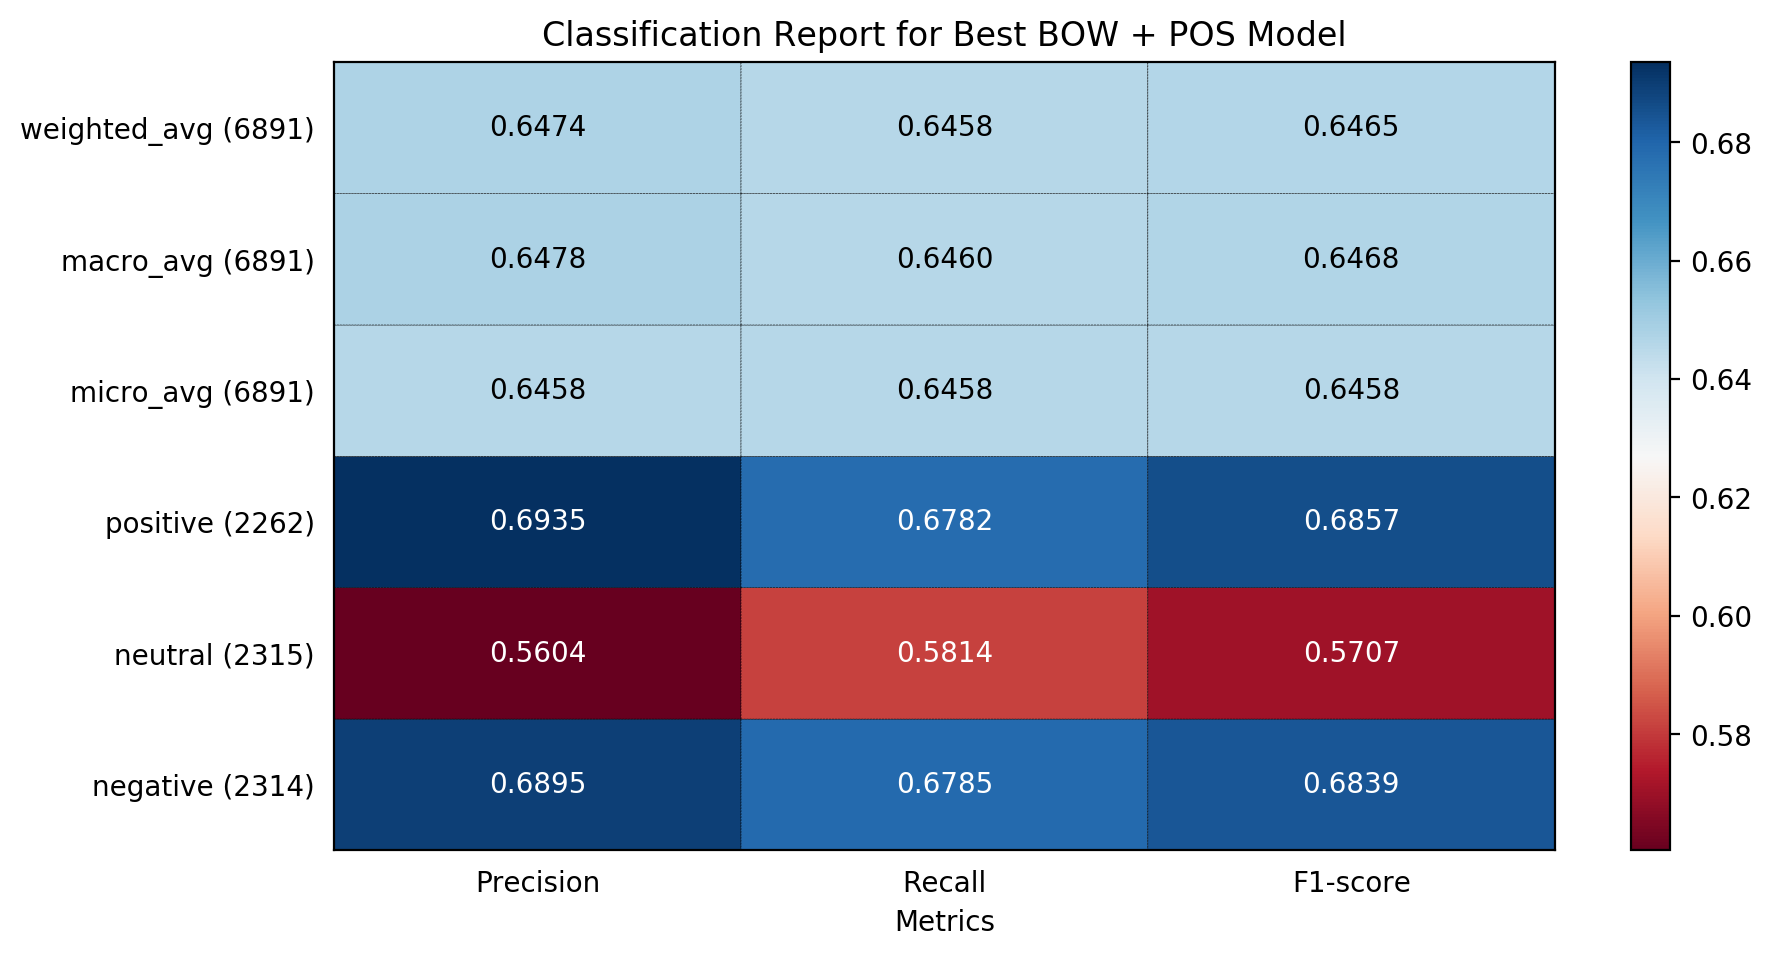
\includegraphics[width=0.8\textwidth]{pics/BOW_POS.png}
\caption{Heat Map for the Classification Report for the Top-Scoring BOW+POS Classifier}
\label{bow_pos}
\end{figure}


   \paragraph{Grouping}
         We have tested both the suggestion from \cite{hatz} to weight just adjectives as well as the one from \cite{pos-based-model} and \cite{benamara}  to combine adjectives and adverbs into one group. Weighting just adjectives yields the F$_{1}$ score of 0.6432\%, which is a slightly better than the 0.6383\%  F$_{1}$ score of the baseline. However, this scheme does not appear in our top results. Combining adjectives and adverbs into one class yields the F$_{1}$ score of 0.6415\%. 
      
      
      \paragraph{Comparison of Results}
   The best weighting combination \citet{improving-sa} achieved with their research did not perform well on our data. None of their top ten configurations scored above the F$_{1}$ score of 0.59 on our dataset. Overall, all other weighting combinations with just POS as features performed equally poorly. 
      
      
\section{Discussion}


   \paragraph{Verdict}
Including POS categories as features on their own do not reach the results of either BOW or TFIDF classifiers. Incorporating POS into BOW improves the scores by about 1\%, which is not a significant value. Hence, we can not generalise that POS categories have a significant impact on SA.

\paragraph{Indicators of Sentiment}

Emoticons alone are already strong predictors of sentiment. Similarly influential is the combination of emoticons and interjections. Adjectives perform not so well in isolation, but consistently receive the strongest weights from high-scoring models. 80 \% of the top ten models do not include nouns and verbs, which suggests that these categories are not crucial to SA. However, one model appears to be an outlier: it assigns the highest weights to nouns, while verbs, adjectives and adverbs all receive significantly lower weights. 

      \paragraph{Differences among the Categories}
Based on the results, one can postulate that the differences in degrees to which POS categories influence the sentiment of a sentence are not definite. The pattern suggests that emoticons and interjections are consistently more important, and adjectives as well as adverbs are also important. In 90\% of cases nouns and verbs play a secondary role. However, one of the top scoring models assigns its highest weight to nouns.

      
   \paragraph{TFIDF}
         The fact that the TFIDF classifier outperforms both BOW and BOW+POS models is consistent with the research done by \cite{Wang2018_WordClustering}, who state that TFIDF is one of the most robust and efficient schemes for feature weighting. 
         
      \paragraph{Issues with POS}
         
         On our dataset the ARK tagger made more mistakes than one would expect, based on its performance in \cite{comparison-taggers} and \cite{cmutagger2-paper}. Among often mistakes are adjectives being tagged as verbs and proper nouns being tagged as nouns or vice versa.
         
         Furthermore, the labelled data is not ideal. Especially the classification of neutral tweets is highly subjective. For example, a tweet that includes the following statement was labelled as neutral by human annotates: \textit{Then again you hate Trump so you prob hate facts}. Our top BOW+POS classifier predicted that the tweet is negative. Arguably, a sentence that contains the word \textit{hate} twice can indeed be classified as negative.
         
        Moreover, POS categories do not account for a variety of issues in any meaningful way. Firstly, only linguistic input has been used for classification. In reality, the tweets often contain images, videos, or links. These could be valuable clues with regards to SA. Secondly, such linguistic phenomenon as sarcasm is still a challenge for SA, especially if the classifiers are not optimised for it. 
   

      		
   \section{Future Work and Conclusion}
   
   \subsection{Future Work}
   Latent features such as POS categories carry valuable information. Therefore, it is reasonable to continue their integration into SA. One approach would be to extend the integration of syntactic categories with semantic categories such as tweet's topic, whether its contents are sarcastic, or whether the tweets include pop-culture references. Also, non-linguistic content such as pictures and videos can be taken into account during classification.
   Furthermore, one could experiment with integrating deep learning systems to discover latent features of terms.
   
   \subsection{Conclusion}
   In our project we have built a POS-enriched SA classifier with adjustable parameters such as the choice of the POS categories to consider, the feature selection cutoff, and the weights for the union of models. The main take-away message is that POS model can slightly improve a BOW classifier by circa 1\%. However, the differences between the performance of BOW, TFIDF, BOW+POS, and BOW+TFIDF+POS models are not significant enough to allow us to state with certainty that POS categories as features improve SA on any dataset.
  
   
\newpage
   \section{Appendix}
   
   \begin{figure}[h]
\centering
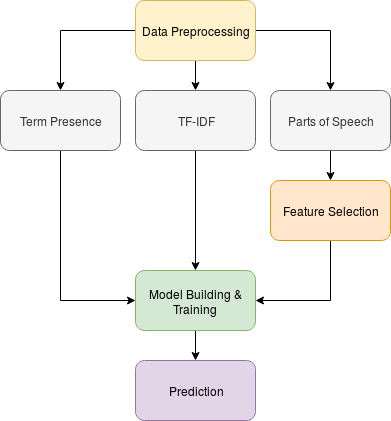
\includegraphics[width=9cm]{pics/pipeline2.png}
    \caption{Pipeline Design}
    \label{pipeline}
\end{figure}

   \begin{figure}[h!]
\centering
   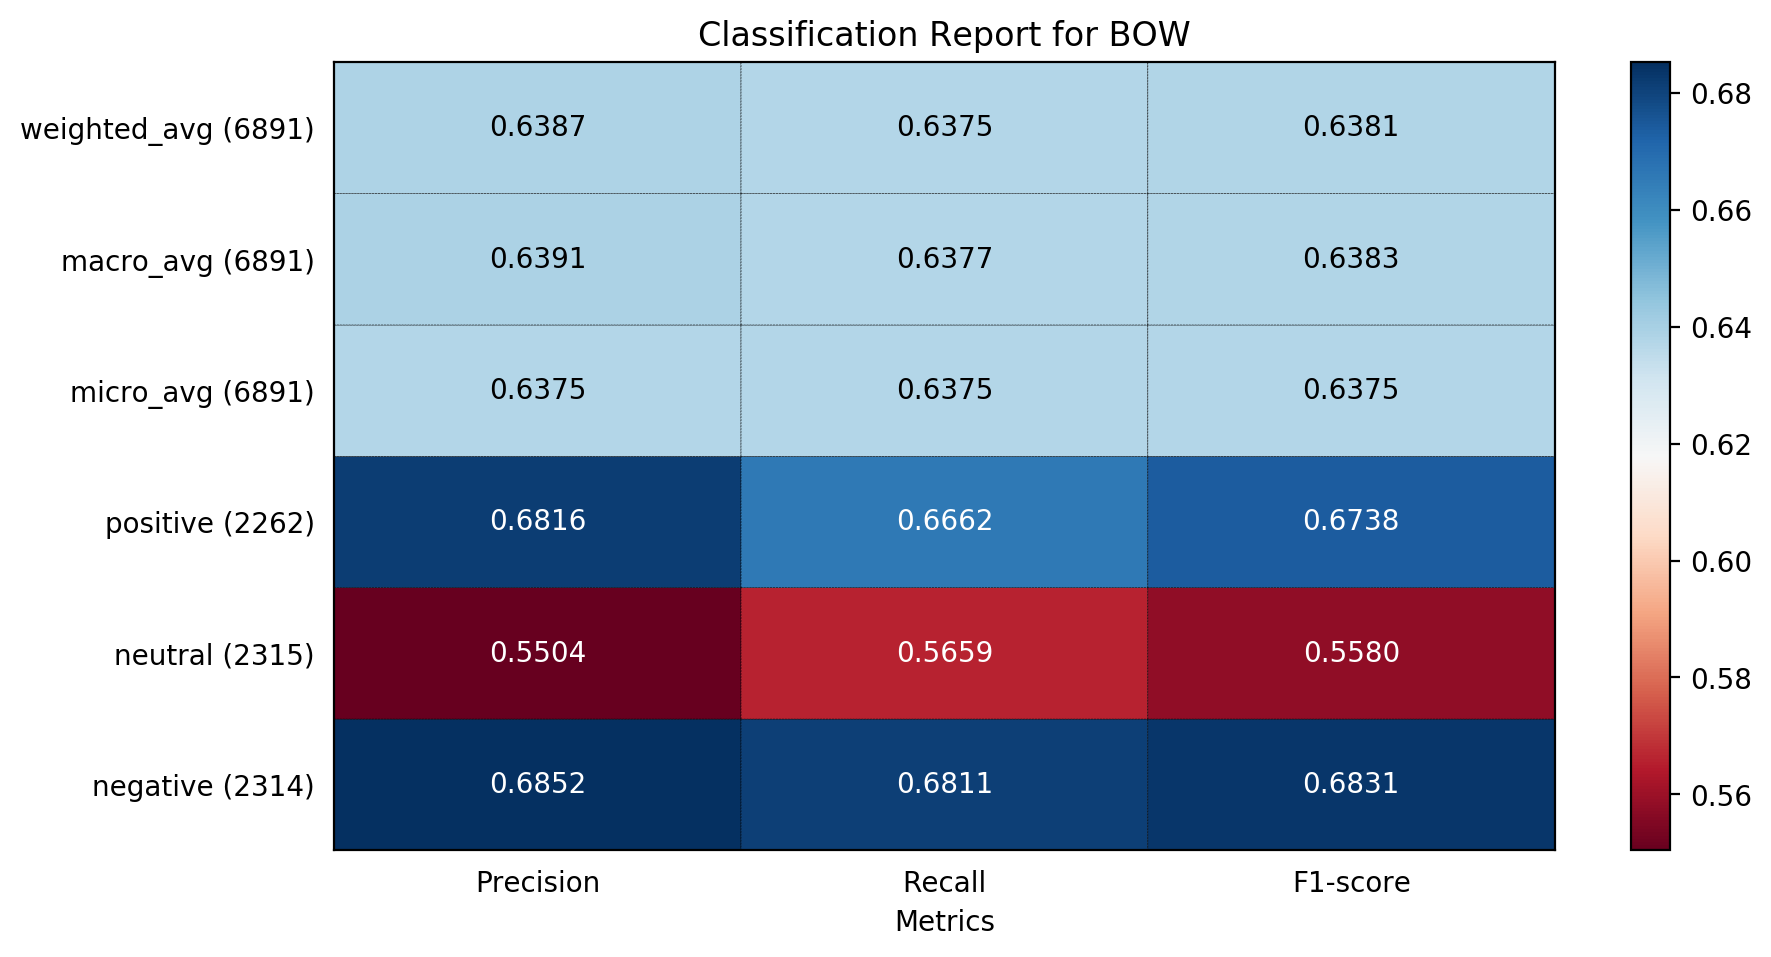
\includegraphics[width=\linewidth]{pics/BOW.png}
    \caption{Heat Map for BOW}
        \label{heat_map_bow}
\end{figure}


  \begin{figure}[h!]
  \centering
 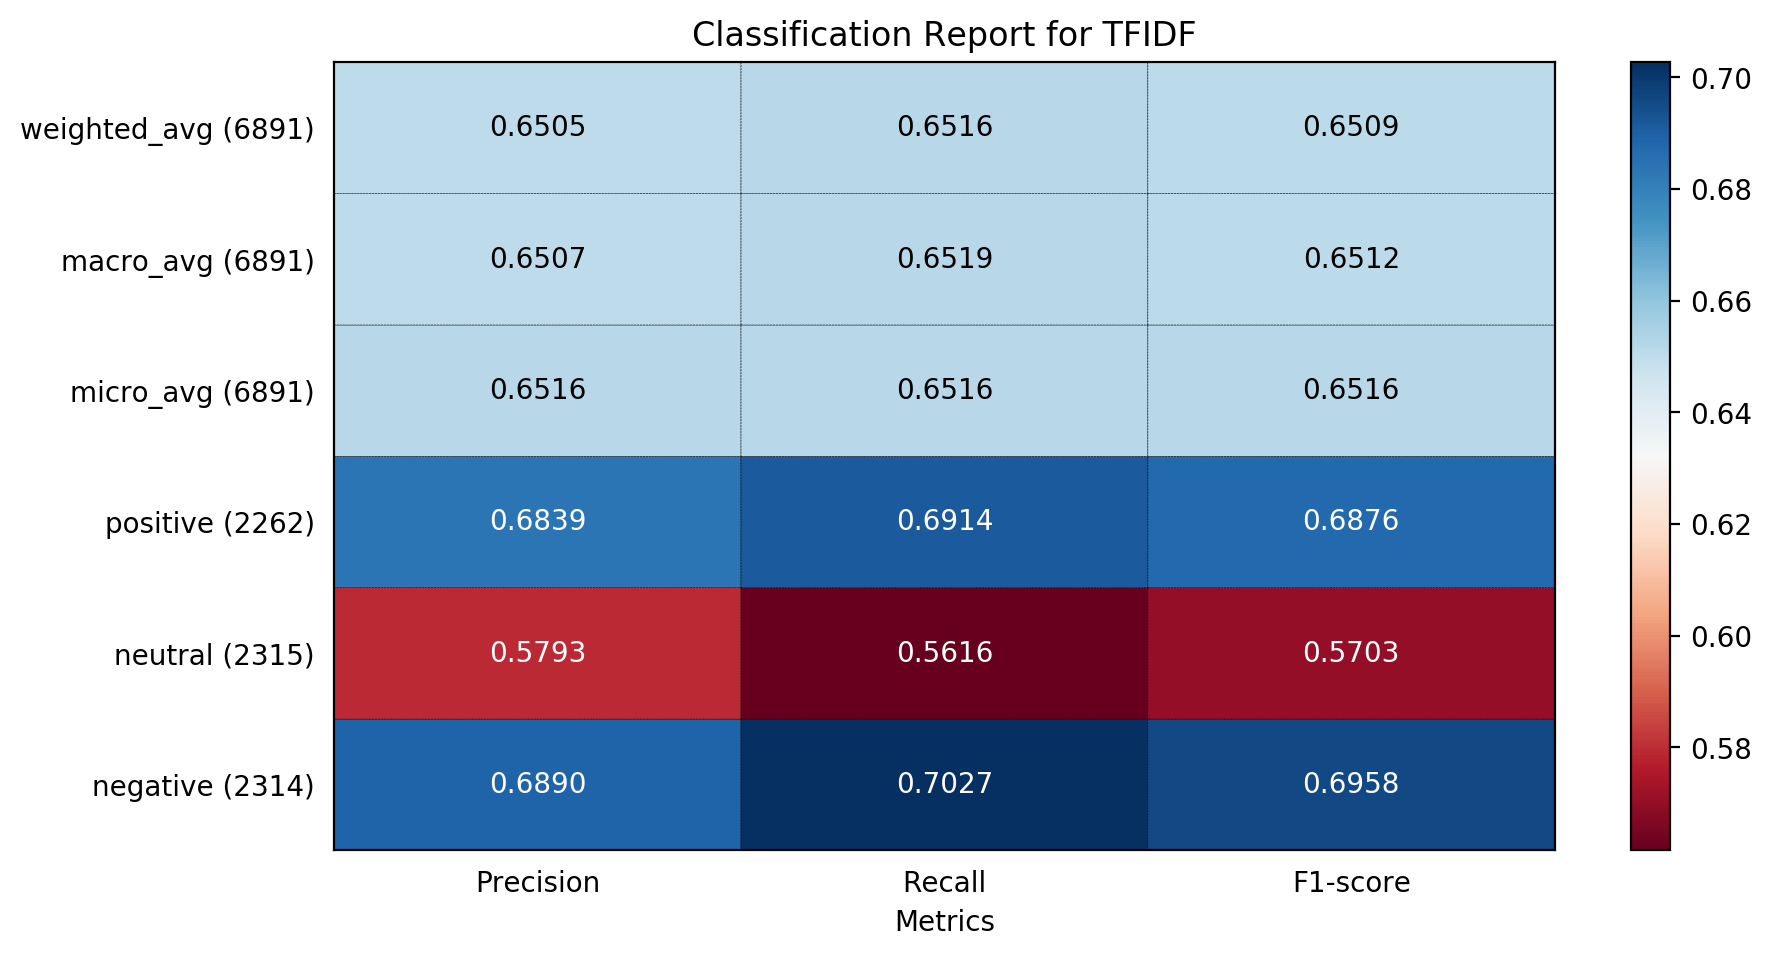
\includegraphics[width=\linewidth]{pics/TFIDF.png}
    \caption{Heat Map for TFIDF}
    \label{heat_map_tfidf}
      \end{figure}
    

  \begin{figure}[h!]
  \centering
 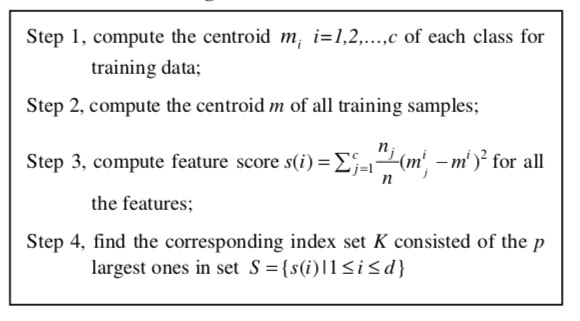
\includegraphics[width=0.7\linewidth]{pics/ocfs.jpeg}
    \caption{Orthogonal Centroid Feature Selection Algorithm}
        \label{ocfs}
      \end{figure}


\newpage

\bibliography{projectbib}

\end{document}